\documentclass[11pt]{article}

\usepackage[margin=1in]{geometry}
\usepackage{amsmath,amsfonts,bm}
\usepackage{array}
\usepackage{booktabs}
\usepackage{caption}
\usepackage{graphicx}
\usepackage{longtable}
\usepackage{placeins}
\usepackage{ragged2e}
\usepackage{xurl}
\usepackage{hyperref}
\hypersetup{hidelinks}

\setlength{\parindent}{0pt}
\setlength{\parskip}{0.45em}
\setlength{\emergencystretch}{3em}
\captionsetup{font=small,labelfont=bf}
\renewcommand{\thefigure}{S\arabic{figure}}
\renewcommand{\thetable}{S\arabic{table}}
\renewcommand{\theequation}{S\arabic{equation}}
\newcommand{\TAMR}{TAMR-DTI}
\newcommand{\R}{\mathbb{R}}
\newcommand{\E}{\mathbb{E}}
\newcommand{\SiLU}{\operatorname{SiLU}}
\newcommand{\softmax}{\operatorname{softmax}}
\newcommand{\LayerNorm}{\operatorname{LayerNorm}}
\newcommand{\MeanPool}{\operatorname{MeanPool}}
\newcommand{\MaskedMean}{\operatorname{MaskedMean}}

\title{\textbf{Supporting Information}\\[4pt]
\large TAMR-DTI: Target-Aware Modulation and Mamba-Based Representation
Refinement for Drug-Target Interaction Prediction}
\author{Wei Li$^{1}$, Wei Liu$^{2*}$, Xiaoqing Hu$^{3*}$, and Shenghui Shi$^{1*}$\\[2pt]
\small $^{1}$Beijing University of Chemical Technology, Beijing, China\\
\small $^{2}$Academy of Military Medical Sciences, Beijing, China\\
\small $^{3}$Peking University Third Hospital, Beijing, China\\[2pt]
\small $^{*}$Corresponding authors: \texttt{liuweilcf@163.com};
\texttt{huxiaoqingbd01@sina.com}; \texttt{shish@mail.buct.edu.cn}}

\begin{document}
\maketitle

\begin{center}
\textit{This file is submitted as Supporting Information and is intended to be
read together with the main manuscript.}
\end{center}

\tableofcontents
\clearpage

\section{Data, Preprocessing, and Reproducibility Details}
\label{si:legacy_details}

This section preserves and expands the data and implementation information from
the previously prepared Supporting Information. It is included so that the new
equation guide and standalone artwork do not remove any reproducibility details
from the earlier SI version.

\subsection{Dataset Sources and Processed Splits}

We evaluate four public drug-target interaction benchmarks: BindingDB,
BioSNAP, Human, and C. elegans. Each sample contains a drug SMILES string, a
protein sequence, and a binary interaction label. The statistics below are
computed from the processed training, validation, and test split files used by
the experiments. The split files are fixed across repeated runs; the seed is
varied for model initialization and training stochasticity.

\begin{table}[!htbp]
\centering
\caption{Processed dataset statistics used by the manuscript.}
\label{tab:si_processed_dataset_stats}
\begin{tabular}{lrrrrrr}
\toprule
Dataset & Drugs & Proteins & Interactions & Positive & Negative & Positive rate \\
\midrule
BindingDB & 14,643 & 2,623 & 49,199 & 20,674 & 28,525 & 42.02\% \\
BioSNAP & 4,505 & 2,181 & 27,464 & 13,830 & 13,634 & 50.36\% \\
Human & 2,726 & 2,001 & 5,997 & 2,633 & 3,364 & 43.91\% \\
C. elegans & 1,767 & 1,876 & 7,786 & 3,893 & 3,893 & 50.00\% \\
\bottomrule
\end{tabular}
\end{table}

\begin{table}[!htbp]
\centering
\caption{Training-split class counts and positive-class weights.}
\label{tab:si_training_weights}
\begin{tabular}{lrrr}
\toprule
Dataset & Training positives & Training negatives & Positive weight $N_-/N_+$ \\
\midrule
BindingDB & 14,583 & 19,856 & 1.3616 \\
BioSNAP & 9,684 & 9,540 & 0.9851 \\
Human & 1,846 & 2,351 & 1.2736 \\
C. elegans & 2,727 & 2,723 & 0.9985 \\
\bottomrule
\end{tabular}
\end{table}

Data access points are listed in the manuscript Data Availability Statement:
BindingDB, BioSNAP, and the Human/C. elegans benchmark files in the
TransformerCPI repository.

\subsection{Input Processing and Feature-Cache Schema}

SMILES strings are encoded by a ChemBERTa hidden-state cache and converted to
DGL molecular graphs. Protein sequences are encoded by a ProtBERT hidden-state
cache. The data loader validates cache shapes and retains explicit masks for
protein residues and invalid conformer slots. The main model uses the vanilla
cache variant, \texttt{drug3d\_features.pt}.

\begin{table}[!htbp]
\centering
\caption{Feature-cache tensors and dimensions.}
\label{tab:si_cache_schema}
\scriptsize
\setlength{\tabcolsep}{3pt}
\begin{tabular}{>{\RaggedRight\arraybackslash}p{0.15\linewidth}>{\RaggedRight\arraybackslash}p{0.24\linewidth}>{\RaggedRight\arraybackslash}p{0.18\linewidth}>{\RaggedRight\arraybackslash}p{0.32\linewidth}}
\toprule
Stream & File or tensor & Shape & Processing and use \\
\midrule
Drug 1D & \texttt{smiles\_features.pt} & $354\times128$ & ChemBERTa token hidden states after adaptive pooling. \\
Drug graph & DGL graph & Up to $290\times75$ & Canonical atom/bond features; self-loops enabled. \\
Drug 3D & \texttt{drug3d\_features.pt} & $K\times64\times128$ & Per-conformer atom features; $K=8$ in the main model. \\
Coordinates & 3D conformer coordinates & $K\times64\times3$ & Coordinates consumed by the EGNN branch. \\
Conformer metadata & \texttt{conf\_mask}, energy & $K$, $K$ & Validity mask and UFF energy for target-aware scoring. \\
Protein & \texttt{protein\_features.pt} & $128\times1024$ & ProtBERT residue features after pooling; residue mask retained. \\
\bottomrule
\end{tabular}
\end{table}

RDKit ETKDGv3 generates up to eight conformers. The extraction routine uses
random seed 42, RMSD pruning threshold 0.5, and one embedding thread. UFF
optimization is attempted for at most 100 iterations when parameters are
available. Molecules with more than 160 heavy atoms are skipped by the 3D
extraction guard. Protein sequences are upper-cased after whitespace removal;
U, Z, O, and B are replaced with X before token encoding. The model-side
protein length is padded or masked to 128. The feature-extraction schema
version is 3.

\subsection{Complete Architecture Configuration}

The model uses a 128-dimensional shared latent space. Protein context first
conditions target-aware conformer scoring. The resulting drug representation
provides a ligand context for FiLM modulation of protein tokens. A
bidirectional protein-side Mamba block refines the protein sequence before
one-layer BiIntention cross-modal matching.

\begin{table}[!htbp]
\centering
\caption{Main TAMR-DTI architecture configuration.}
\label{tab:si_architecture_config}
\scriptsize
\setlength{\tabcolsep}{4pt}
\begin{tabular}{>{\RaggedRight\arraybackslash}p{0.25\linewidth}>{\RaggedRight\arraybackslash}p{0.64\linewidth}}
\toprule
Component & Setting \\
\midrule
Drug graph encoder & Input node dimension 75; hidden dimensions [128, 128, 128]; maximum graph length 290. \\
Target-aware conformer encoder & EGNN dimension 128; $K=8$; 64 atoms per conformer; protein-conditioned score input; energy projection included. \\
Drug fusion & Graph and conformer tokens form 354 structural slots; layer-normalized fusion with a learned sigmoid gate initialized at bias $-2.0$. \\
Protein encoder & 1024-dimensional ProtBERT features projected to 128; three ProteinACmix layers; kernels 3, 6, 9; eight heads; ligand FiLM scale 0.05. \\
Protein Mamba & Protein tokens only; bidirectional; $d_{\rm state}=16$; $d_{\rm conv}=4$; expansion 2; dropout 0.1; Mamba-1 backend; gate bias $-2.0$. \\
BiIntention & One layer; eight heads; embedding dimension 128; bidirectional drug-protein intention updates. \\
Prediction head & Four-layer MLP; input 256; hidden 256; intermediate output 128; binary logit output. \\
\bottomrule
\end{tabular}
\end{table}

\subsection{Training, Loss, and Evaluation}

\begin{table}[!htbp]
\centering
\caption{Training and evaluation settings.}
\label{tab:si_training_evaluation}
\scriptsize
\setlength{\tabcolsep}{4pt}
\begin{tabular}{>{\RaggedRight\arraybackslash}p{0.28\linewidth}>{\RaggedRight\arraybackslash}p{0.59\linewidth}}
\toprule
Setting & Value \\
\midrule
Optimizer & Adam \\
Initial learning rate & $1\times10^{-4}$ \\
Weight decay & $1\times10^{-4}$ \\
Maximum epochs & 100 \\
Batch and accumulation & 16 per GPU; gradient accumulation 4 steps \\
Gradient clipping & Maximum norm 1.0 \\
Scheduler & Plateau; factor 0.5; patience 5; minimum learning rate $1\times10^{-6}$ \\
Early stopping & Patience 10; minimum improvement $1\times10^{-4}$ \\
Checkpoint & Highest validation AUROC \\
Runtime & Python 3.9; PyTorch, DeepSpeed ZeRO-2, DGL/DGLLife, RDKit, Transformers, and mamba-ssm; eight Tesla P100 GPUs. \\
\bottomrule
\end{tabular}
\end{table}

For completeness, the threshold-dependent metrics used in the manuscript are
defined below. The threshold $\tau$ is applied to the predicted probability.
\begin{align}
\mathrm{Accuracy}(\tau)
 &= \frac{\mathrm{TP}(\tau)+\mathrm{TN}(\tau)}
 {\mathrm{TP}(\tau)+\mathrm{TN}(\tau)+\mathrm{FP}(\tau)+\mathrm{FN}(\tau)},\\
\mathrm{Precision}(\tau)
 &= \frac{\mathrm{TP}(\tau)}{\mathrm{TP}(\tau)+\mathrm{FP}(\tau)},\\
\mathrm{Recall}(\tau)
 &= \frac{\mathrm{TP}(\tau)}{\mathrm{TP}(\tau)+\mathrm{FN}(\tau)},\\
\mathrm{F1}(\tau)
 &= \frac{2\,\mathrm{Precision}(\tau)\,\mathrm{Recall}(\tau)}
 {\mathrm{Precision}(\tau)+\mathrm{Recall}(\tau)}.
\end{align}
The validation threshold is searched over $0.01,0.02,\ldots,0.99$ and then
applied unchanged to the held-out test split. Fixed-threshold results use
$\tau=0.5$.

\subsection{Main Run Matrix}

All four datasets use the same main architecture and five fixed seeds, 42
through 46. Configuration identifiers correspond to files under
\texttt{configs/experiments/}.

\begin{table}[!htbp]
\centering
\caption{Main repeated-seed configuration index.}
\label{tab:si_run_matrix}
\scriptsize
\setlength{\tabcolsep}{5pt}
\begin{tabular}{lll}
\toprule
Dataset & Seed & Configuration \\
\midrule
BindingDB & 42 & \texttt{stage2\_main\_01} \\
BindingDB & 43 & \texttt{stage2\_main\_02} \\
BindingDB & 44 & \texttt{stage2\_main\_03} \\
BindingDB & 45 & \texttt{stage2\_main\_04} \\
BindingDB & 46 & \texttt{stage2\_main\_05} \\
BioSNAP & 42 & \texttt{stage2\_main\_06} \\
BioSNAP & 43 & \texttt{stage2\_main\_07} \\
BioSNAP & 44 & \texttt{stage2\_main\_08} \\
BioSNAP & 45 & \texttt{stage2\_main\_09} \\
BioSNAP & 46 & \texttt{stage2\_main\_10} \\
Human & 42 & \texttt{stage2\_main\_11} \\
Human & 43 & \texttt{stage2\_main\_12} \\
Human & 44 & \texttt{stage2\_main\_13} \\
Human & 45 & \texttt{stage2\_main\_14} \\
Human & 46 & \texttt{stage2\_main\_15} \\
C. elegans & 42 & \texttt{stage2\_main\_16} \\
C. elegans & 43 & \texttt{stage2\_main\_17} \\
C. elegans & 44 & \texttt{stage2\_main\_18} \\
C. elegans & 45 & \texttt{stage2\_main\_19} \\
C. elegans & 46 & \texttt{stage2\_main\_20} \\
\bottomrule
\end{tabular}
\end{table}

\subsection{Expanded Performance and Diagnostic Results}

The standalone tables in Section~\ref{si:tables} reproduce the main
AUROC/AUPRC comparison, the repeated-run summary, the BioSNAP module ablation,
and the conformer-count diagnostic. All diagnostics use BioSNAP, seed 42, the
same fixed split, validation-AUROC checkpoint selection, and fixed-threshold
evaluation. They are single-seed mechanism diagnostics rather than repeated-run
significance tests.

\subsection{Conformer-Weight and Mamba Interpretability}

The analysis uses all 5,493 BioSNAP test pairs from the seed-42 target-aware
model. For each sample, conformer weights are sorted in descending order, and
prediction groups use validation threshold 0.62. Normalized conformer entropy is
calculated as
\begin{equation}
\bar H_i=-\frac{1}{\log K_i}\sum_{k=1}^{K_i}w_{ik}\log(w_{ik}+\epsilon),
\end{equation}
where $K_i$ is the number of valid conformers for sample $i$ and $\epsilon$ is
a numerical-stability constant.

\begin{table}[!htbp]
\centering
\caption{Population-level interpretability statistics.}
\label{tab:si_interpretability_statistics}
\scriptsize
\setlength{\tabcolsep}{4pt}
\begin{tabular}{lrrrr}
\toprule
Group & $n$ & Top-1 weight & Entropy & Mamba refine mean \\
\midrule
All test pairs & 5,493 & 0.5975 & 0.4799 & 0.094526 \\
True positive & 2,175 & $0.5910\pm0.2341$ & $0.4876\pm0.2545$ & 0.093963 \\
True negative & 2,328 & $0.5974\pm0.2311$ & $0.4808\pm0.2517$ & 0.095077 \\
False positive & 417 & $0.5857\pm0.2287$ & $0.4834\pm0.2468$ & 0.093675 \\
False negative & 573 & $0.6309\pm0.2401$ & $0.4446\pm0.2651$ & 0.095047 \\
\bottomrule
\end{tabular}
\end{table}

\begin{table}[!htbp]
\centering
\caption{Median sorted conformer weights by prediction group.}
\label{tab:si_sorted_conformer_weights}
\begin{tabular}{lrrrr}
\toprule
Group & Rank 1 & Rank 2 & Rank 3 & Rank 4 \\
\midrule
True positive & 0.5320 & 0.2479 & 0.0946 & 0.0121 \\
True negative & 0.5288 & 0.2457 & 0.0964 & 0.0137 \\
False positive & 0.5192 & 0.2579 & 0.1036 & 0.0132 \\
False negative & 0.5804 & 0.2317 & 0.0756 & 0.0053 \\
\bottomrule
\end{tabular}
\end{table}

\begin{table}[!htbp]
\centering
\caption{Auxiliary modulation statistics from the interpretability analysis.}
\label{tab:si_auxiliary_modulation}
\begin{tabular}{lr}
\toprule
Quantity & Mean \\
\midrule
Mamba gate & 0.132949 \\
Conformer top-1 margin & 0.365227 \\
Protein FiLM layer 1 strength & 0.020351 \\
Protein FiLM layer 2 strength & 0.013285 \\
Protein FiLM layer 3 strength & 0.012323 \\
\bottomrule
\end{tabular}
\end{table}

The sample-level analysis file is
\url{outputs/interpretability/biosnap_seed42/biosnap_seed42_interpretability_samples.csv}.
It records prediction groups, threshold, conformer entropy, top-1 weight,
conformer margin, Mamba summaries, eight conformer weights, and layer-wise FiLM
statistics.

\subsection{Reproducibility and Availability}

The implementation, preprocessing code, and experiment configuration files are
available at \url{https://github.com/leleleocc/TAMR-DTI}. Model code is under
\texttt{src/}, feature extraction is under \texttt{scripts/pre\_extract.py},
and the run configurations listed in Table~\ref{tab:si_run_matrix} are under
\texttt{configs/experiments/}. To reproduce a run, obtain the public benchmark
files, construct the fixed split directory with \texttt{train.csv},
\texttt{val.csv}, and \texttt{test.csv}, build the ChemBERTa, ProtBERT, graph,
and 3D caches with the settings above, and launch the corresponding
configuration. Select the checkpoint by validation AUROC and evaluate the
held-out test set under the metric conventions in this SI and the manuscript.

\section{Equation and Notation Guide}
\label{si:equation_guide}

This section provides an equation-by-equation reading guide for Section 3
(Methodology) of the main manuscript. The equation identifiers in the first
column are the labels used in the manuscript source. The table is deliberately
redundant with the prose description so that every tensor, mask, gate, and
aggregation operation can be checked without searching through the main text.

\subsection{Global conventions and dimensions}

Bold upper-case symbols denote matrices or token sequences, bold lower-case
symbols denote vectors, and plain lower-case symbols denote scalars. A batch
dimension is omitted unless it is needed for interpretation. The principal
dimensions of the reported configuration are listed below.

\begin{table}[!htbp]
\centering
\caption{Global dimensions and fixed configuration used by TAMR-DTI.}
\label{tab:si_dimensions}
\small
\begin{tabular}{>{\RaggedRight\arraybackslash}p{0.28\linewidth}>{\RaggedRight\arraybackslash}p{0.18\linewidth}>{\RaggedRight\arraybackslash}p{0.44\linewidth}}
\toprule
Symbol or setting & Value & Interpretation \\
\midrule
$d$ & 128 & Shared hidden dimension for drug and protein tokens. \\
$N_g$ & 290 & Padded graph-token count. \\
$N_c$ & 64 & Resampled atom-token count per conformer. \\
$K$ & 8 & Number of conformer slots in the main model. \\
$L_d$ & 354 & Drug-token length, $N_g+N_c$. \\
$L_p$ & Variable & Protein-token length after padding and masking. \\
$d_c$ & Backbone-dependent & ChemBERTa hidden size before pooling. \\
$H$ & 8 & Number of heads in the BiIntention module. \\
ProteinACmix layers & 3 & Ligand-conditioned protein encoder depth. \\
BiIntention layers & 1 & Pairwise interaction depth in the main model. \\
\bottomrule
\end{tabular}
\end{table}

The mask $m_j\in\{0,1\}$ indicates whether protein position $j$ is a valid
residue. The conformer-validity indicator $q_k\in\{0,1\}$ indicates whether
conformer slot $k$ contains a generated geometry. Concatenation is written with
square brackets; $\odot$ is element-wise multiplication; $[\,;\,]$ denotes
feature concatenation; $\sigma$ is the sigmoid; $\operatorname{LN}$ denotes
layer normalization; and $(\cdot)^\dagger$ denotes the Moore--Penrose
pseudoinverse.

\subsection{Section 3 equation map}

\renewcommand{\arraystretch}{1.25}
\scriptsize
\setlength{\tabcolsep}{2pt}
\begin{longtable}{>{\RaggedRight\arraybackslash}p{0.20\linewidth}>{\RaggedRight\arraybackslash}p{0.28\linewidth}>{\RaggedRight\arraybackslash}p{0.18\linewidth}>{\RaggedRight\arraybackslash}p{0.28\linewidth}}
\caption{Equation-by-equation explanation for the Methodology section of the main manuscript.}\label{tab:si_equation_guide}\\
\toprule
Main-text label & Compact form & Main objects and dimensions & Role in the computation \\
\midrule
\endfirsthead
\multicolumn{4}{c}{\tablename\ \thetable{} -- continued from previous page}\\
\toprule
Main-text label & Compact form & Main objects and dimensions & Role in the computation \\
\midrule
\endhead
\midrule
\multicolumn{4}{r}{Continued on next page}\\
\endfoot
\bottomrule
\endlastfoot

\texttt{dti\_prediction} & $s=f_\theta(D,T)$; $p=\sigma(s)$; $\hat y=\mathbf{1}[p\ge\tau]$ & $s,p,\tau,\hat y$ are scalars & Converts a drug--target pair into a logit, probability, and thresholded prediction. \\
\texttt{overall\_pipeline} & $\mathbf D\to\mathbf x_D\to\mathbf P\to\mathbf P'\to\mathbf f\to s$ & $\mathbf D\in\R^{L_d\times d}$; $\mathbf P\in\R^{L_p\times d}$; $\mathbf f\in\R^{2d}$ & Gives the order of the complete forward pass and makes the two conditioning directions explicit. \\
\texttt{chemberta\_encoding} & $\mathbf U^{\rm chem}=\operatorname{ChemBERTa}(s_D)$ & $\mathbf U^{\rm chem}\in\R^{L_s\times d_c}$ & Encodes the SMILES string with the frozen molecular language model. \\
\texttt{chemberta\_pooling} & $\mathbf X_{\rm chem}=\operatorname{Pool}_{L_d,d}(\mathbf U^{\rm chem}_{\neg\rm special})$ & $\mathbf X_{\rm chem}\in\R^{L_d\times d}$ & Removes special tokens and maps variable-length language features to the fixed drug-token interface. \\
\texttt{gcn\_projection} & $\mathbf h_i^{g,0}=\mathbf W_g\mathbf a_i$ & $\mathbf a_i\in\R^{75}$; $\mathbf h_i^{g,0}\in\R^d$ & Projects atom descriptors into the shared hidden space; the padding indicator is prevented from adding atom semantics. \\
\texttt{gcn\_output} & $\mathbf H^g=\operatorname{GCN}(\mathcal G_D,\mathbf H^{g,0})$ & $\mathbf H^g\in\R^{N_g\times d}$ & Aggregates local bond and neighborhood information into graph tokens. \\
\texttt{egnn\_conformer} & $(\mathbf Z_k,\mathbf R'_k)=\operatorname{EGNN}(\mathbf F_k,\mathbf R_k)$ & $\mathbf F_k\in\R^{N_c\times d}$; $\mathbf R_k\in\R^{N_c\times3}$ & Updates conformer atom features while respecting Euclidean coordinate transformations. \\
\texttt{conformer\_global} & $\mathbf c_k=N_c^{-1}\sum_i\mathbf z_{k,i}$ & $\mathbf c_k\in\R^d$ & Produces one global summary per conformer for target-aware scoring; atom-level features are retained separately. \\
\texttt{protein\_seed\_projection} & $\mathbf P^0=\mathbf W_p\operatorname{LN}(\mathbf P_{\rm ProtBERT})$ & $1024\to d$; $\mathbf P^0\in\R^{L_p\times d}$ & Places ProtBERT residue features in the same hidden space used by the drug branches. \\
\texttt{protein\_context} & $\mathbf x_T=\frac{\sum_jm_j\mathbf p^0_j}{\max(1,\sum_jm_j)}$ & $\mathbf x_T\in\R^d$ & Computes the masked protein context that conditions conformer selection. \\
\texttt{conformer\_score} & $a_k=\mathbf w_a^\top\SiLU(\mathbf W_a[\mathbf c_k;\mathbf x_T;\mathbf u_k]+\mathbf b_a)+b_s$ & $a_k\in\R$; $\mathbf u_k=\mathbf W_e\epsilon_k$ & Scores each candidate geometry using its content, target context, and normalized energy. \\
\texttt{conformer\_weight} & $\alpha_k=\frac{e^{a_k}q_k}{\sum_\ell e^{a_\ell}q_\ell}$ & $\boldsymbol\alpha\in\R^K$ & Normalizes scores over valid conformers; invalid slots receive no probability mass. \\
\texttt{target\_aware\_3d} & $\mathbf Z^{3D}=\sum_k\alpha_k\mathbf Z_k$; $\mathbf c^{3D}=\sum_k\alpha_k\mathbf c_k$ & $\mathbf Z^{3D}\in\R^{N_c\times d}$; $\mathbf c^{3D}\in\R^d$ & Forms the protein-conditioned atom-level and global 3D representations. \\
\texttt{geo\_concat} & $\mathbf X_{\rm str}=[\mathbf H^g;\mathbf Z^{3D}]$ & $\mathbf X_{\rm str}\in\R^{(N_g+N_c)\times d}$ & Concatenates topology and target-aware geometry to match the ChemBERTa token length. \\
\texttt{drug\_gate} & $\mathbf D=\mathbf G^D\odot\widetilde{\mathbf X}_{\rm chem}+(1-\mathbf G^D)\odot\widetilde{\mathbf X}_{\rm str}$ & $\mathbf G^D\in(0,1)^{L_d\times d}$ & Learns a slot- and channel-wise balance between semantic and structural drug streams. \\
\texttt{drug\_context} & $\mathbf x_D=L_d^{-1}\sum_i\mathbf d_i$ & $\mathbf x_D\in\R^d$ & Summarizes the fused drug tokens and sends ligand context to the protein encoder. \\
\texttt{protein\_ffn\_half\_1} & $\mathbf U^\ell=\tfrac12\operatorname{FFN}_1^\ell(\mathbf P^{\ell-1})+\tfrac12\mathbf P^{\ell-1}$ & $\mathbf U^\ell\in\R^{L_p\times d}$ & Applies a conservative first feed-forward residual update in ProteinACmix layer $\ell$. \\
\texttt{film\_params} & $[\boldsymbol\gamma^\ell,\boldsymbol\beta^\ell]=\operatorname{MLP}_{\rm film}^\ell(\mathbf x_D)$ & $\boldsymbol\gamma^\ell,\boldsymbol\beta^\ell\in\R^d$ & Generates ligand-dependent feature-wise scale and shift parameters; $\rho=0.05$ limits their initial effect. \\
\texttt{ligand\_film} & $\widetilde{\mathbf U}^\ell=\mathbf U^\ell\odot(1+\bar{\boldsymbol\gamma}^\ell)+\bar{\boldsymbol\beta}^\ell$ & Broadcast over $L_p$ residue tokens & Modulates protein features with the fused ligand context. \\
\texttt{protein\_acmix} & $\mathbf A^\ell=\operatorname{MHSA}_{rel}(\widetilde{\mathbf U}^\ell)+\widetilde{\mathbf U}^\ell$; $\mathbf C^\ell=\operatorname{Conv}(\mathbf A^\ell)+\mathbf A^\ell$ & All tensors are $L_p\times d$ & Combines long-range relative attention, local convolution, and a second half-step FFN. \\
\texttt{protein\_output} & $\mathbf P=\mathbf P^3$ & $\mathbf P\in\R^{L_p\times d}$ & Defines the ligand-conditioned protein sequence passed to refinement. \\
\texttt{feature\_projection} & $\psi_{\rm chem}:\R^{128}\to\R^{128}$; $\psi_g:\R^{75}\to\R^{128}$; $\psi_p:\R^{1024}\to\R^{128}$ & Three active input mappings & Records the shared-dimension contract between cached features and trainable encoders. \\
\texttt{feature\_contexts} & $\mathbf x_T=\operatorname{MaskedMean}(\mathbf P^0,\mathbf m)$; $\mathbf x_D=\operatorname{MeanPool}(\mathbf D)$ & Two vectors in $\R^d$ & Documents the order of the two feedback paths: target-to-drug first, then drug-to-protein. \\
\texttt{protein\_masked\_input} & $\mathbf p^{mask}_j=m_j\mathbf p_j$ & $\mathbf P^{mask}\in\R^{L_p\times d}$ & Suppresses padded residue positions before protein-side Mamba processing. \\
\texttt{bidirectional\_mamba} & $\mathbf M=\mathbf W_m[\mathbf M_f;\mathbf M_b]$ & $\mathbf M_f$ and $\mathbf M_b$ are forward/backward Mamba streams & Captures ordered protein dependencies in both sequence directions; the backward stream is computed on the reversed sequence. \\
\texttt{mamba\_residual} & $\mathbf R=\mathbf P^{mask}+\operatorname{Dropout}(\mathbf M)$; $\bar{\mathbf P}_{\rm Mamba}=\mathbf R+\operatorname{FFN}_m(\mathbf R)$ & $L_p\times d$ & Adds residual and feed-forward refinement, then reapplies the residue mask. \\
\texttt{mamba\_gate} & $g=\sigma(\eta)$; $\mathbf P'=\mathbf P+g(\mathbf P_{\rm Mamba}-\mathbf P)$ & $g\in(0,1)$; $\mathbf P'\in\R^{L_p\times d}$ & Controls the strength of Mamba injection; $\eta=-2$ initializes $g\approx0.119$. \\
\texttt{bi\_self\_attention} & $\mathbf D^s=\operatorname{SA}_D(\mathbf D)$; $\mathbf P^s=\operatorname{SA}_P(\mathbf P')$ & Drug and protein streams retain their lengths & Refines each modality independently before cross-modal intention updates. \\
\texttt{intention\_head} & $\mathbf Q_r=\mathbf Q\mathbf W_r^Q$; $\mathbf K_r=\mathbf X\mathbf W_r^K$; $\mathbf V_r=\mathbf X\mathbf W_r^V$ & $d_h=d/H$ per head & Builds a feature-space interaction map using a ridge-stabilized pseudoinverse and head weighting. \\
\texttt{intention\_block} & $\Phi(\mathbf X,\mathbf Q)=\beta\mathbf Q^\top\softmax(\operatorname{Int}(\operatorname{LN}(\mathbf X),\mathbf Q))$ & $\Phi\in\R^{d\times d}$ & Converts cross-modal intention features into a compact pair representation. \\
\shortstack[l]{\texttt{bidirectional\_intention\_}\\\texttt{update}} & $\mathbf V_p^\ell=\Phi(\mathbf D^{\ell-1},\mathbf P^{\ell-1})$; $\mathbf V_d^\ell=\Phi(\mathbf P^{\ell-1},\mathbf D^{\ell-1})$ & Drug and protein directions are computed separately & Keeps the interaction update bidirectional rather than concatenating unimodal features. \\
\texttt{fusion\_pooling} & $\mathbf f=[\operatorname{MaxPool}(\mathbf D^{(L)});\operatorname{MaxPool}(\mathbf P^{(L)})]$ & $\mathbf f\in\R^{2d}=\R^{256}$ & Produces the fixed-size pair vector consumed by the prediction head. \\
\texttt{prediction\_mlp} & $\mathbf f\to\mathbf z_1\to\mathbf z_2\to\mathbf z_3\to s$ & $256\to256\to256\to128\to1$ & Maps the pair vector to one interaction logit using ReLU and layer normalization. \\
\texttt{weighted\_bce} & $\mathcal L=-B^{-1}\sum_i[w_+y_i\log p_i+(1-y_i)\log(1-p_i)]$ & $B$ samples; $w_+>0$ & Optimizes the logit-derived probability while compensating for positive/negative imbalance. \\
\texttt{pos\_weight} & $w_+=N_-/N_+$ & Training-split counts only & Computes the dataset-specific positive-class weight without using validation or test labels. \\
\end{longtable}

\subsection{Interpretation of the conditioning order}

The key implementation contract is the order of operations. ProtBERT features
are projected and masked to form $\mathbf x_T$, which scores and aggregates
the candidate conformers. The resulting fused drug sequence is pooled to form
$\mathbf x_D$, which then modulates the protein sequence through FiLM. Mamba is
applied only to the ordered protein stream, after ligand conditioning and before
BiIntention. This order should be preserved when reproducing the model; moving
the two context vectors or applying the Mamba block to the drug slots changes
the stated architecture.

The conformer energy $\epsilon_k$ is an auxiliary ranking feature. It is not
treated as a calibrated thermodynamic free energy and is not compared across
molecules as an absolute physical quantity. Invalid conformers are masked in
the softmax, and the implementation activates the first slot as a fallback if
all conformer-validity indicators are zero.

\section{Standalone Tables}
\label{si:tables}

The following tables are supplied as standalone, selectable-text versions for
reviewer inspection and high-resolution reading. They reproduce the numerical
values reported in the manuscript and add no new statistical claims. The
equation guide and the machine-readable data/code links in the manuscript
should be used for interpretation and reuse.

\begin{table}[!htbp]
\centering
\caption{Dataset statistics used in the main experiments. Counts are computed from the processed training, validation, and test split files used in this study.}
\label{tab:si_dataset_overview}
\begin{tabular}{lrrrrrr}
\toprule
Dataset & Drugs & Proteins & Interactions & Positive & Negative & Positive rate \\
\midrule
BindingDB & 14,643 & 2,623 & 49,199 & 20,674 & 28,525 & 42.02\% \\
BioSNAP & 4,505 & 2,181 & 27,464 & 13,830 & 13,634 & 50.36\% \\
Human & 2,726 & 2,001 & 5,997 & 2,633 & 3,364 & 43.91\% \\
C. elegans & 1,767 & 1,876 & 7,786 & 3,893 & 3,893 & 50.00\% \\
\bottomrule
\end{tabular}
\end{table}

\begin{table}[!htbp]
\centering
\caption{Basic training hyperparameters for the main experiments.}
\label{tab:si_training_hyperparameters}
\begin{tabular}{>{\RaggedRight\arraybackslash}p{0.40\linewidth}>{\RaggedRight\arraybackslash}p{0.42\linewidth}}
\toprule
Hyperparameter & Value \\
\midrule
Optimizer & Adam \\
Initial learning rate & $1\times10^{-4}$ \\
Weight decay & $1\times10^{-4}$ \\
Maximum epochs & 100 \\
Micro-batch size & 16 per GPU \\
Gradient accumulation & 4 steps \\
Gradient clipping & 1.0 \\
Learning-rate decay factor & 0.5 \\
Minimum learning rate & $1\times10^{-6}$ \\
\bottomrule
\end{tabular}
\end{table}

\begin{table}[!htbp]
\centering
\caption{Dataset-specific positive-class weights used by the binary cross-entropy loss.}
\label{tab:si_dataset_pos_weight}
\begin{tabular}{lrrr}
\toprule
Dataset & Training positives & Training negatives & Positive-class weight \\
\midrule
BindingDB & 14,583 & 19,856 & 1.3616 \\
BioSNAP & 9,684 & 9,540 & 0.9851 \\
Human & 1,846 & 2,351 & 1.2736 \\
C. elegans & 2,727 & 2,723 & 0.9985 \\
\bottomrule
\end{tabular}
\end{table}

\clearpage
\begin{table}[!htbp]
\centering
\caption{AUROC/AUPRC comparison on four benchmark datasets. Baseline values are adopted from reported results; TAMR-DTI values are from five-seed runs and are shown as mean $\pm$ standard deviation.}
\label{tab:si_baseline_landscape}
\scriptsize
\setlength{\tabcolsep}{2.3pt}
\resizebox{\linewidth}{!}{%
\begin{tabular}{lcccccccc}
\toprule
 & \multicolumn{2}{c}{BindingDB} & \multicolumn{2}{c}{BioSNAP} & \multicolumn{2}{c}{Human} & \multicolumn{2}{c}{C. elegans} \\
\cmidrule(lr){2-3}\cmidrule(lr){4-5}\cmidrule(lr){6-7}\cmidrule(lr){8-9}
Method & AUROC & AUPRC & AUROC & AUPRC & AUROC & AUPRC & AUROC & AUPRC \\
\midrule
SVM & $0.904\pm0.002$ & $0.865\pm0.001$ & $0.819\pm0.045$ & $0.839\pm0.038$ & $0.913\pm0.012$ & $0.905\pm0.001$ & $0.925\pm0.009$ & $0.907\pm0.002$ \\
RF & $0.942\pm0.001$ & $0.923\pm0.001$ & $0.857\pm0.009$ & $0.872\pm0.006$ & $0.939\pm0.009$ & $0.927\pm0.001$ & $0.935\pm0.009$ & $0.931\pm0.001$ \\
KNN & $0.895\pm0.001$ & $0.865\pm0.002$ & $0.842\pm0.003$ & $0.805\pm0.003$ & $0.915\pm0.002$ & $0.902\pm0.002$ & $0.912\pm0.003$ & $0.896\pm0.002$ \\
LR & $0.916\pm0.003$ & $0.884\pm0.002$ & $0.821\pm0.004$ & $0.796\pm0.002$ & $0.895\pm0.003$ & $0.862\pm0.001$ & $0.892\pm0.002$ & $0.883\pm0.003$ \\
GraphDTA & $0.944\pm0.004$ & $0.925\pm0.006$ & $0.871\pm0.004$ & $0.870\pm0.006$ & $0.965\pm0.003$ & $0.955\pm0.003$ & $0.959\pm0.004$ & $0.951\pm0.002$ \\
DrugBAN & $0.952\pm0.001$ & $0.936\pm0.001$ & $0.902\pm0.001$ & $0.905\pm0.002$ & $0.979\pm0.001$ & $0.969\pm0.005$ & $0.981\pm0.002$ & $0.978\pm0.002$ \\
IIFDTI & $0.924\pm0.002$ & $0.901\pm0.004$ & $0.895\pm0.003$ & $0.898\pm0.005$ & $0.977\pm0.003$ & $0.967\pm0.027$ & $0.984\pm0.002$ & $0.979\pm0.002$ \\
TransformerCPI & $0.895\pm0.002$ & $0.861\pm0.003$ & $0.843\pm0.008$ & $0.859\pm0.007$ & $0.956\pm0.005$ & $0.943\pm0.002$ & $0.975\pm0.003$ & $0.975\pm0.002$ \\
MolTrans & $0.935\pm0.003$ & $0.901\pm0.004$ & $0.879\pm0.006$ & $0.882\pm0.006$ & $0.979\pm0.003$ & $0.975\pm0.002$ & $0.982\pm0.002$ & $0.979\pm0.002$ \\
BINDTI & $0.956\pm0.001$ & $0.942\pm0.002$ & $0.895\pm0.003$ & $0.894\pm0.003$ & $0.980\pm0.001$ & $0.975\pm0.004$ & $0.985\pm0.002$ & $0.984\pm0.002$ \\
LDM-DTI & $0.960\pm0.002$ & $0.945\pm0.002$ & $0.908\pm0.003$ & $0.906\pm0.003$ & $0.981\pm0.001$ & $0.976\pm0.002$ & $0.988\pm0.002$ & $0.986\pm0.002$ \\
TAMR-DTI & \textbf{$0.964\pm0.001$} & \textbf{$0.954\pm0.002$} & \textbf{$0.930\pm0.002$} & \textbf{$0.935\pm0.002$} & \textbf{$0.982\pm0.002$} & \textbf{$0.978\pm0.002$} & \textbf{$0.992\pm0.001$} & \textbf{$0.991\pm0.001$} \\
\bottomrule
\end{tabular}}
\end{table}

\begin{table}[!htbp]
\centering
\caption{TAMR-DTI repeated-run summary across the four benchmark datasets. Values are mean $\pm$ standard deviation over seeds 42, 43, 44, 45, and 46.}
\label{tab:si_tamr_main_summary}
\scriptsize
\setlength{\tabcolsep}{5pt}
\begin{tabular}{lcccc}
\toprule
Dataset & AUROC & AUPRC & Acc@0.5 & F1@0.5 \\
\midrule
BindingDB & \textbf{$0.964\pm0.001$} & \textbf{$0.954\pm0.002$} & \textbf{$0.909\pm0.003$} & \textbf{$0.891\pm0.004$} \\
BioSNAP & \textbf{$0.930\pm0.002$} & \textbf{$0.935\pm0.002$} & \textbf{$0.857\pm0.004$} & \textbf{$0.859\pm0.004$} \\
Human & \textbf{$0.982\pm0.002$} & \textbf{$0.978\pm0.002$} & \textbf{$0.930\pm0.009$} & \textbf{$0.924\pm0.009$} \\
C. elegans & \textbf{$0.992\pm0.001$} & \textbf{$0.991\pm0.001$} & \textbf{$0.961\pm0.004$} & \textbf{$0.961\pm0.004$} \\
\bottomrule
\end{tabular}
\end{table}

\begin{table}[!htbp]
\centering
\caption{Single-seed diagnostic ablation results on BioSNAP. All variants use seed 42, the same split, validation-AUROC checkpoint selection, and fixed-threshold Acc@0.5/F1@0.5.}
\label{tab:si_biosnap_ablation}
\scriptsize
\setlength{\tabcolsep}{4pt}
\begin{tabular}{lcccc}
\toprule
Variant & AUROC & AUPRC & Acc@0.5 & F1@0.5 \\
\midrule
Full TAMR-DTI & \textbf{0.933} & \textbf{0.937} & \textbf{0.862} & \textbf{0.864} \\
w/o Target-aware conformer & 0.916 & 0.922 & 0.844 & 0.845 \\
w/o Protein FiLM & 0.920 & 0.924 & 0.842 & 0.844 \\
w/o Protein Mamba refinement & 0.918 & 0.925 & 0.842 & 0.845 \\
w/o Bidirectional modulation & 0.920 & 0.926 & 0.848 & 0.849 \\
\bottomrule
\end{tabular}
\end{table}

\clearpage
\begin{table}[!htbp]
\centering
\caption{Single-seed conformer-count comparison on BioSNAP. Conformers are energy-sorted during preprocessing; $n=1$ keeps the lowest-energy conformer only, while larger $n$ values expose additional geometries.}
\label{tab:si_biosnap_conformer_comparison}
\scriptsize
\setlength{\tabcolsep}{3.2pt}
\resizebox{\linewidth}{!}{%
\begin{tabular}{lccrrrrr}
\toprule
Variant & Effective conformers & Aggregation & Best epoch & AUROC & AUPRC & Acc@0.5 & F1@0.5 \\
\midrule
$n=1$ target-aware & 1 & Target-aware & 46 & 0.9277 & 0.9297 & 0.8578 & 0.8591 \\
$n=2$ target-aware & 2 & Target-aware & 68 & 0.9300 & 0.9322 & 0.8575 & 0.8605 \\
$n=4$ target-aware & 4 & Target-aware & 46 & 0.9297 & 0.9345 & 0.8524 & 0.8542 \\
$n=8$ target-aware & 8 & Target-aware & 51 & \textbf{0.9322} & \textbf{0.9356} & 0.8575 & 0.8624 \\
$n=16$ target-aware & 16 & Target-aware & 62 & 0.9312 & 0.9326 & \textbf{0.8631} & \textbf{0.8668} \\
$n=8$ uniform average & 8 & Uniform average & 64 & 0.9308 & 0.9340 & 0.8589 & 0.8616 \\
\bottomrule
\end{tabular}}
\end{table}

\FloatBarrier

\section{High-Resolution Figures}
\label{si:figures}

The figures below are included directly from the original vector PDF artwork in
the manuscript source. Text, lines, and plotted curves therefore remain
selectable and are not rasterized by this SI compilation. The figure numbering
is local to the SI (Figures S1--S7); the corresponding main-text figure labels
are given in each caption.

\begin{figure}[p]
\centering
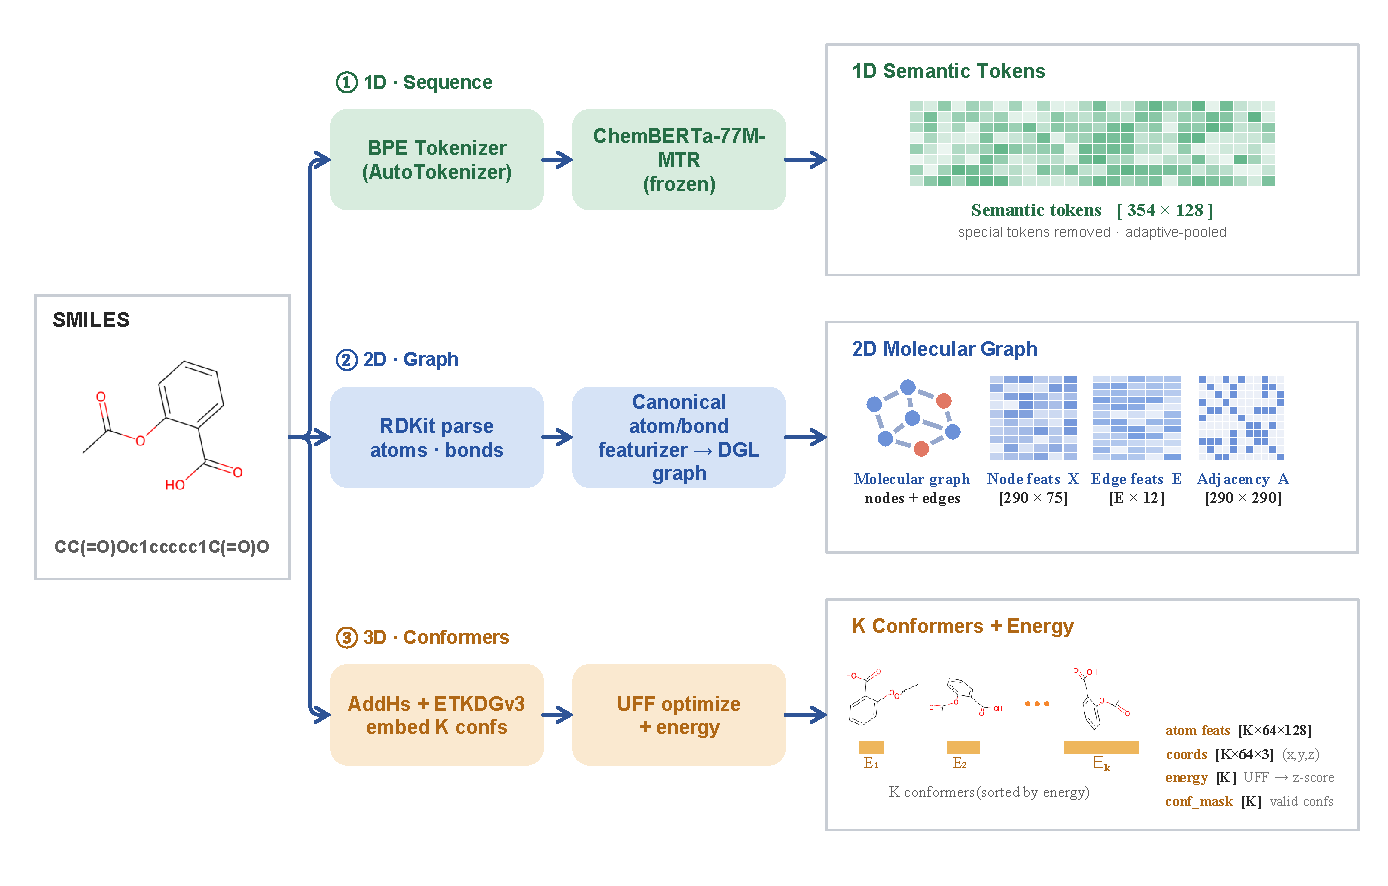
\includegraphics[width=0.98\textwidth,height=0.78\textheight,keepaspectratio]{figures/drug_preprocess.pdf}
\caption{High-resolution version of main-text Figure 1: drug data preprocessing. Starting from a SMILES string, TAMR-DTI constructs a ChemBERTa semantic-token matrix, an RDKit/DGL molecular graph, and a set of energy-ranked 3D conformers with atom features, coordinates, energies, and conformer-validity indicators.}
\label{fig:si_drug_preprocess}
\end{figure}
\clearpage

\begin{figure}[p]
\centering
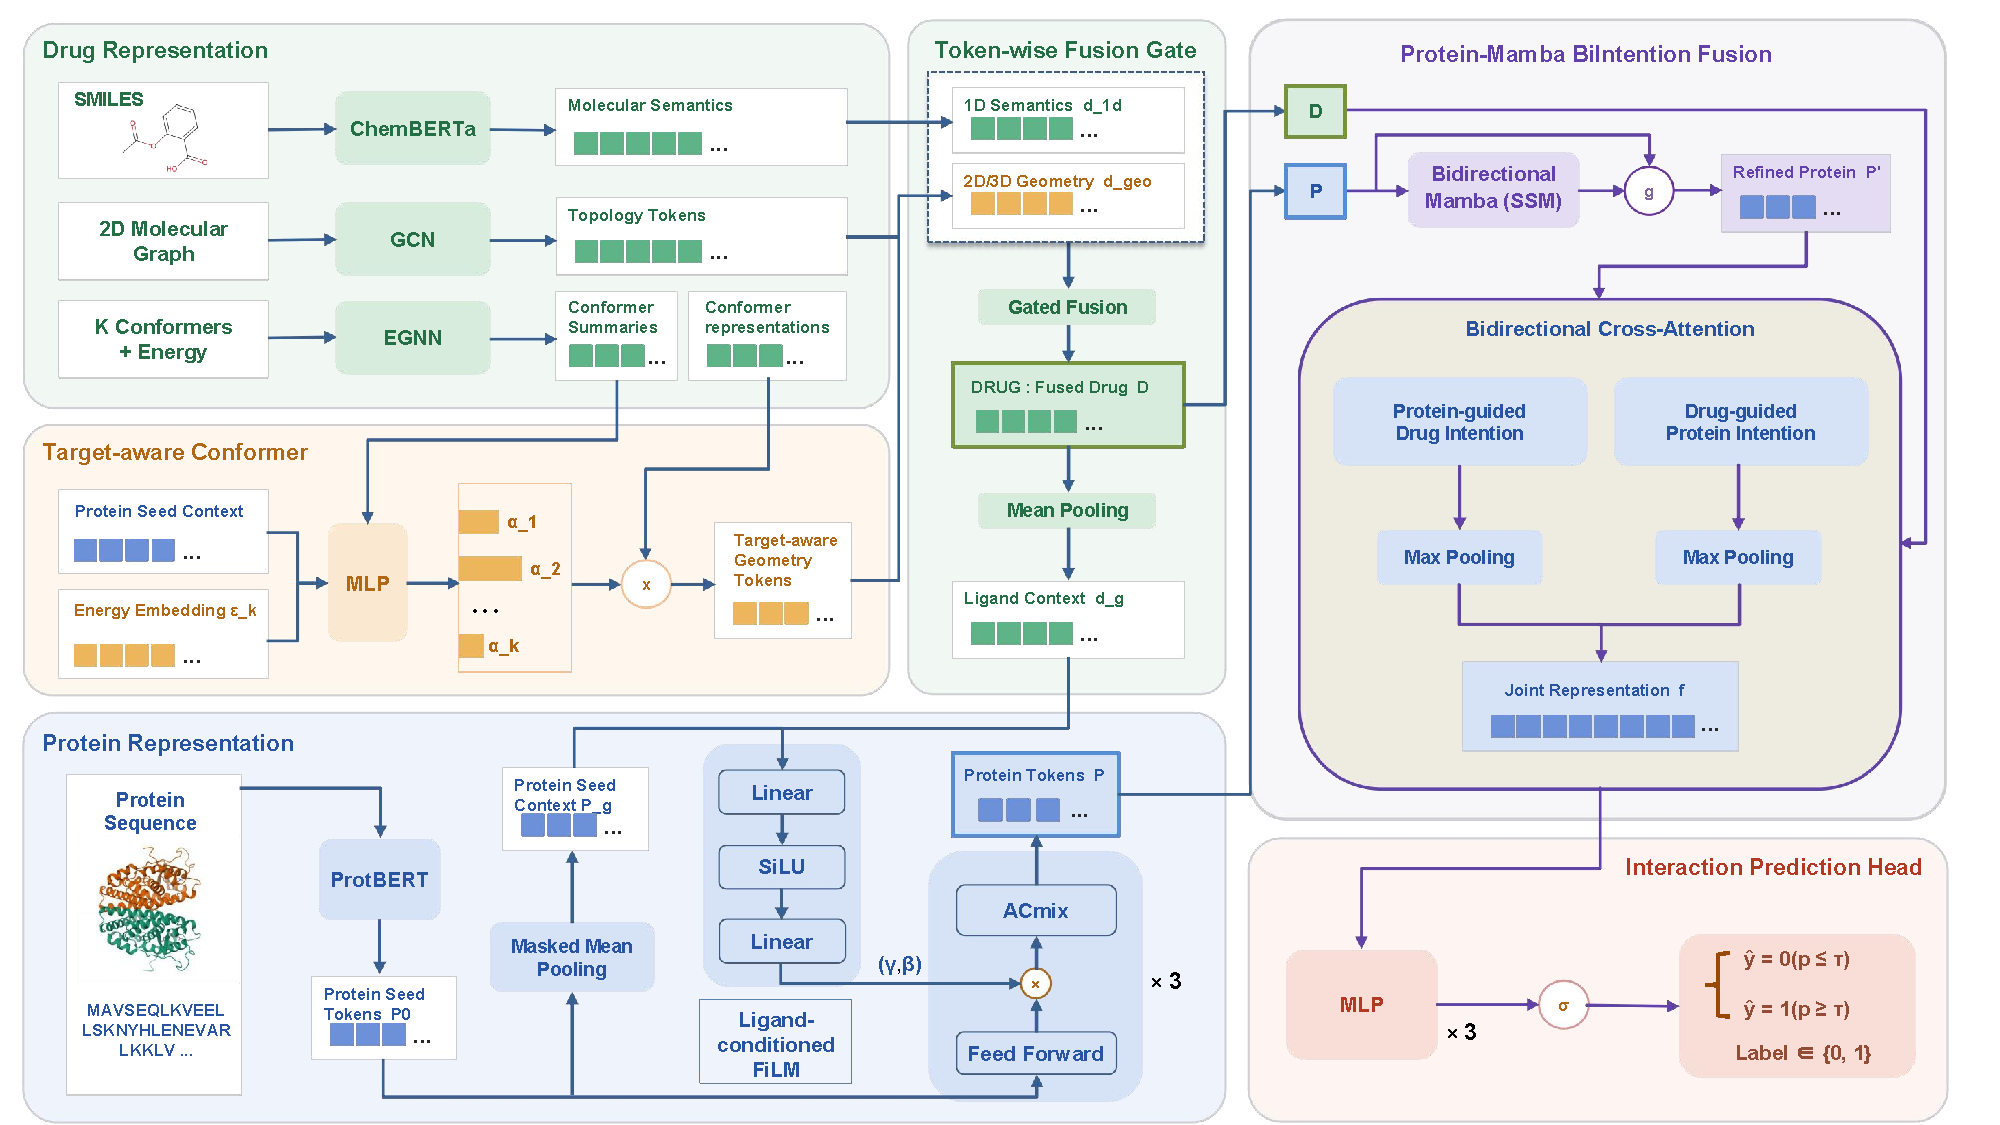
\includegraphics[width=0.98\textwidth,height=0.78\textheight,keepaspectratio]{figures/tamr_dti_architecture.pdf}
\caption{High-resolution version of main-text Figure 2: TAMR-DTI representation framework. The artwork shows the drug representation streams, ligand-conditioned protein representation module, protein-side refinement block, and BiIntention interaction head.}
\label{fig:si_tamr_dti_architecture}
\end{figure}
\clearpage

\begin{figure}[p]
\centering
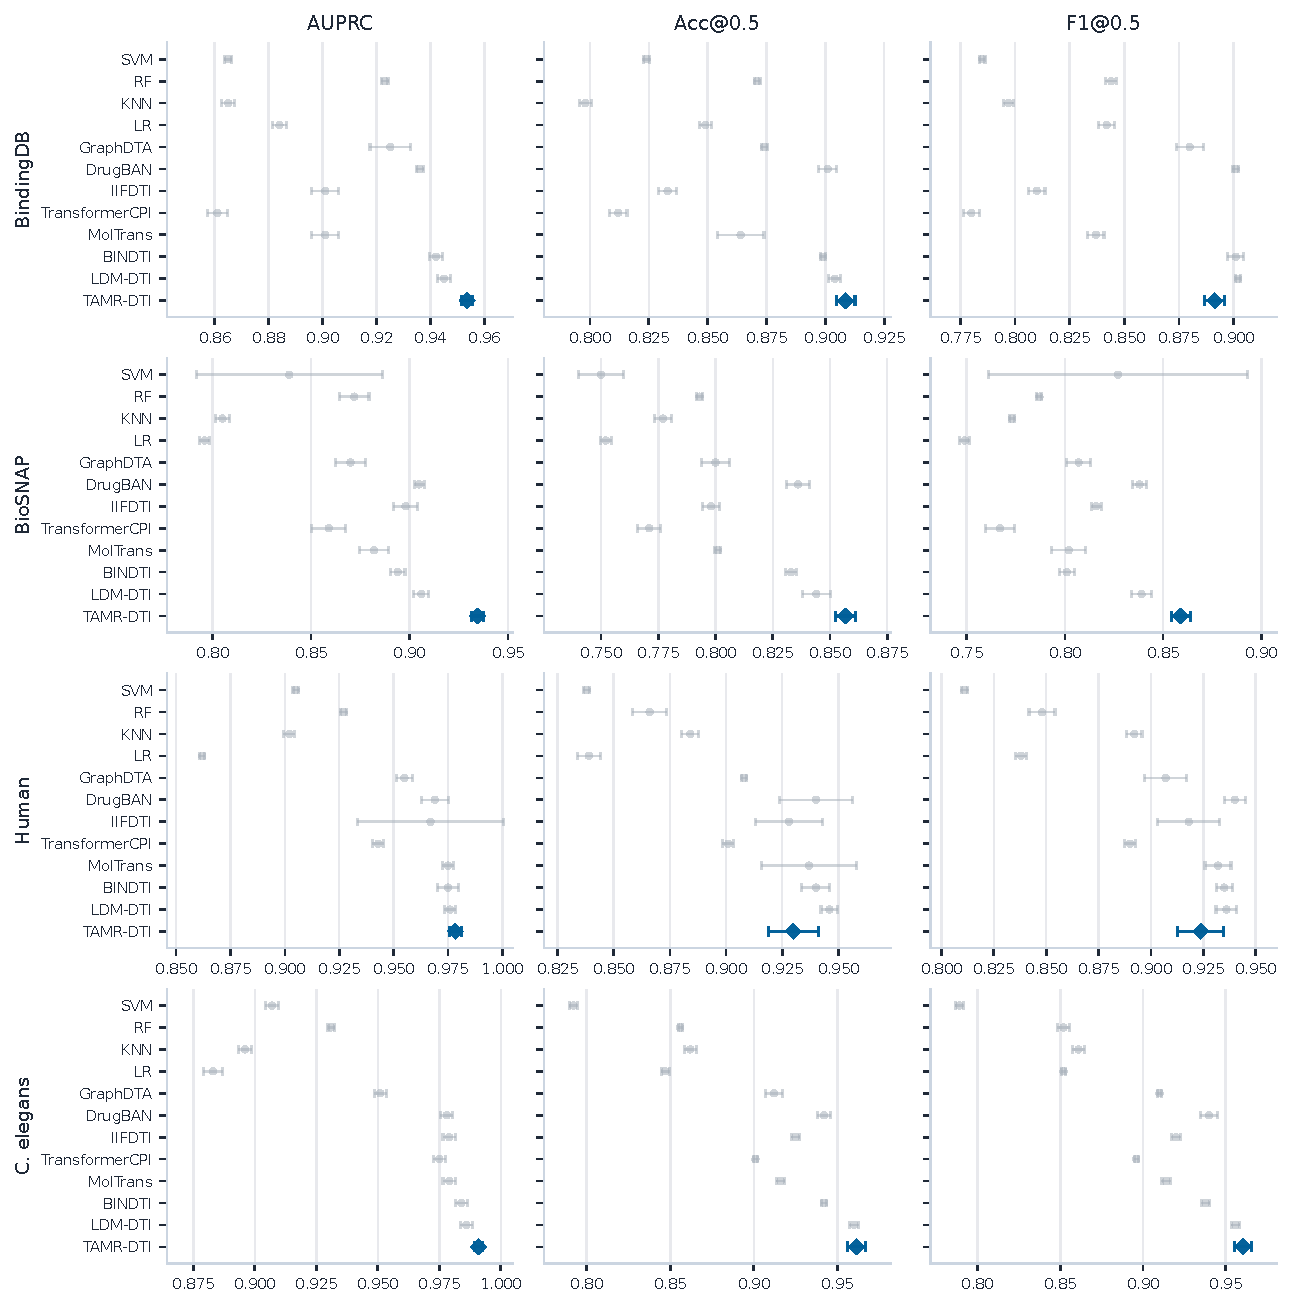
\includegraphics[width=0.98\textwidth,height=0.78\textheight,keepaspectratio]{figures/all_method_ci_comparison.pdf}
\caption{High-resolution version of the main-text all-method comparison figure. The plot shows metric values and uncertainty intervals for AUROC, AUPRC, Acc@0.5, and F1@0.5 across the four benchmark datasets.}
\label{fig:si_all_method_ci_comparison}
\end{figure}
\clearpage

\begin{figure}[p]
\centering
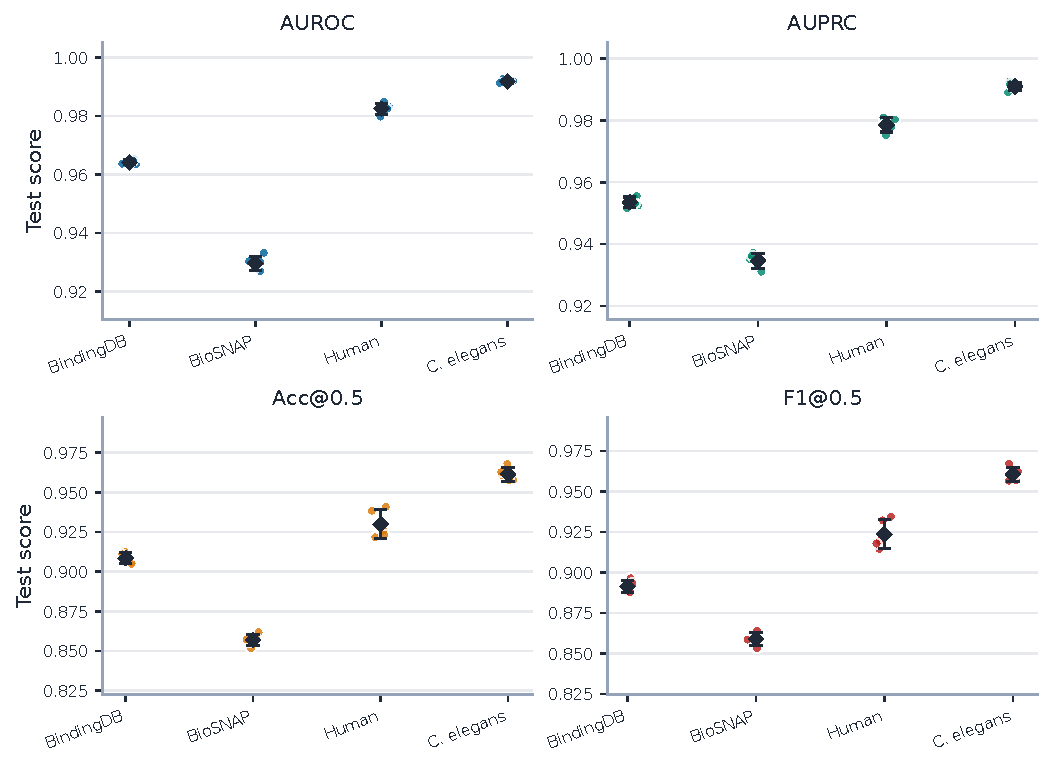
\includegraphics[width=0.98\textwidth,height=0.78\textheight,keepaspectratio]{figures/main_seed_stability.pdf}
\caption{High-resolution version of the main-text seed-stability figure. Each point represents one fixed-seed run and the intervals summarize the repeated-run variation under the stated evaluation protocol.}
\label{fig:si_main_seed_stability}
\end{figure}
\clearpage

\begin{figure}[p]
\centering
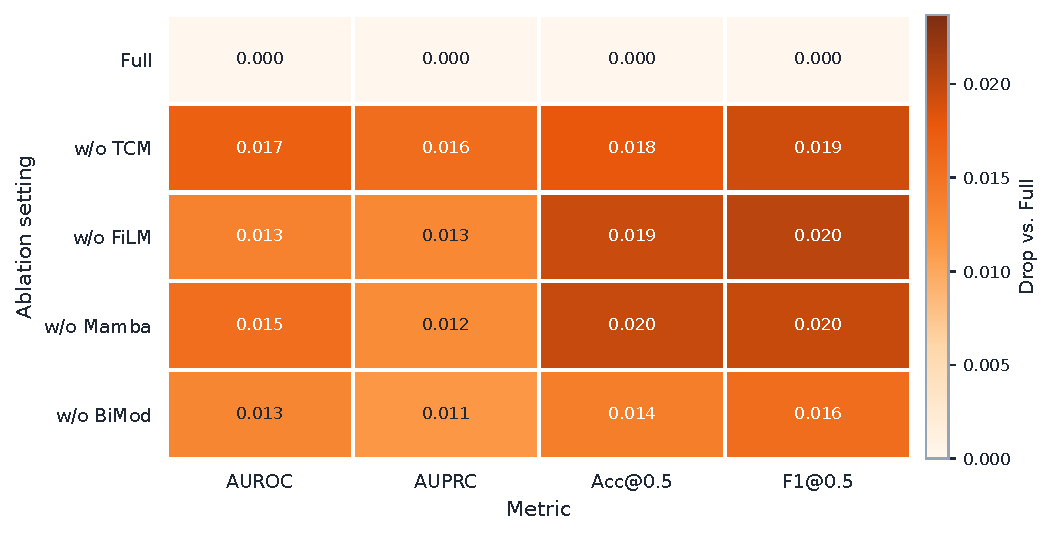
\includegraphics[width=0.98\textwidth,height=0.78\textheight,keepaspectratio]{figures/ablation_biosnap_seed42_drop.pdf}
\caption{High-resolution version of the main-text BioSNAP ablation-drop figure. Each cell reports the relative test-score decrease caused by removing one module under the same seed, split, checkpoint selection rule, and fixed threshold; the complete model is the zero-drop reference.}
\label{fig:si_biosnap_ablation_drop}
\end{figure}
\clearpage

\begin{figure}[p]
\centering
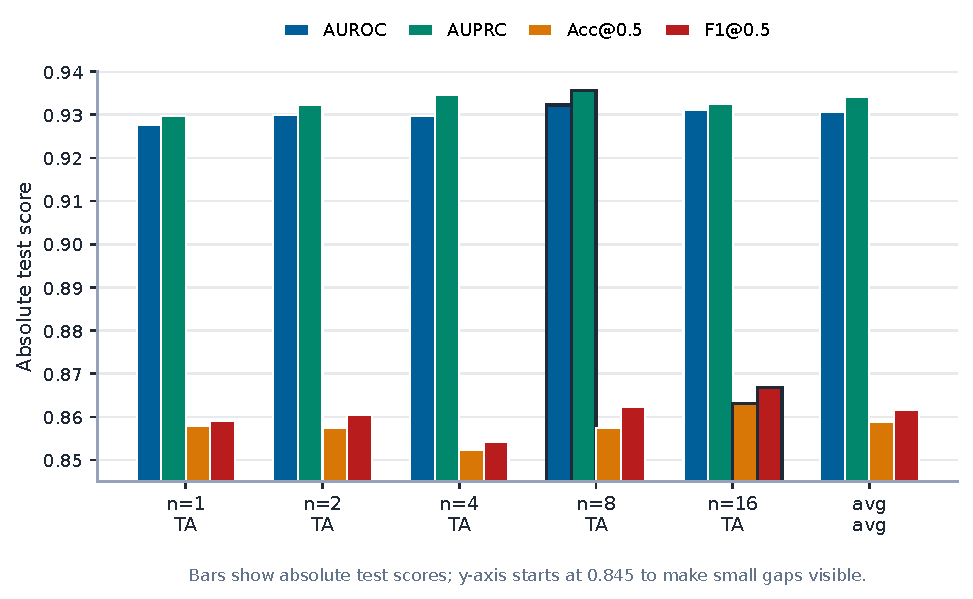
\includegraphics[width=0.98\textwidth,height=0.78\textheight,keepaspectratio]{figures/conformer_biosnap_seed42_comparison.pdf}
\caption{High-resolution version of the main-text conformer-count comparison figure. The plot compares effective conformer counts and uniform versus target-aware aggregation on BioSNAP under the single-seed diagnostic protocol.}
\label{fig:si_biosnap_conformer_comparison}
\end{figure}
\clearpage

\begin{figure}[p]
\centering
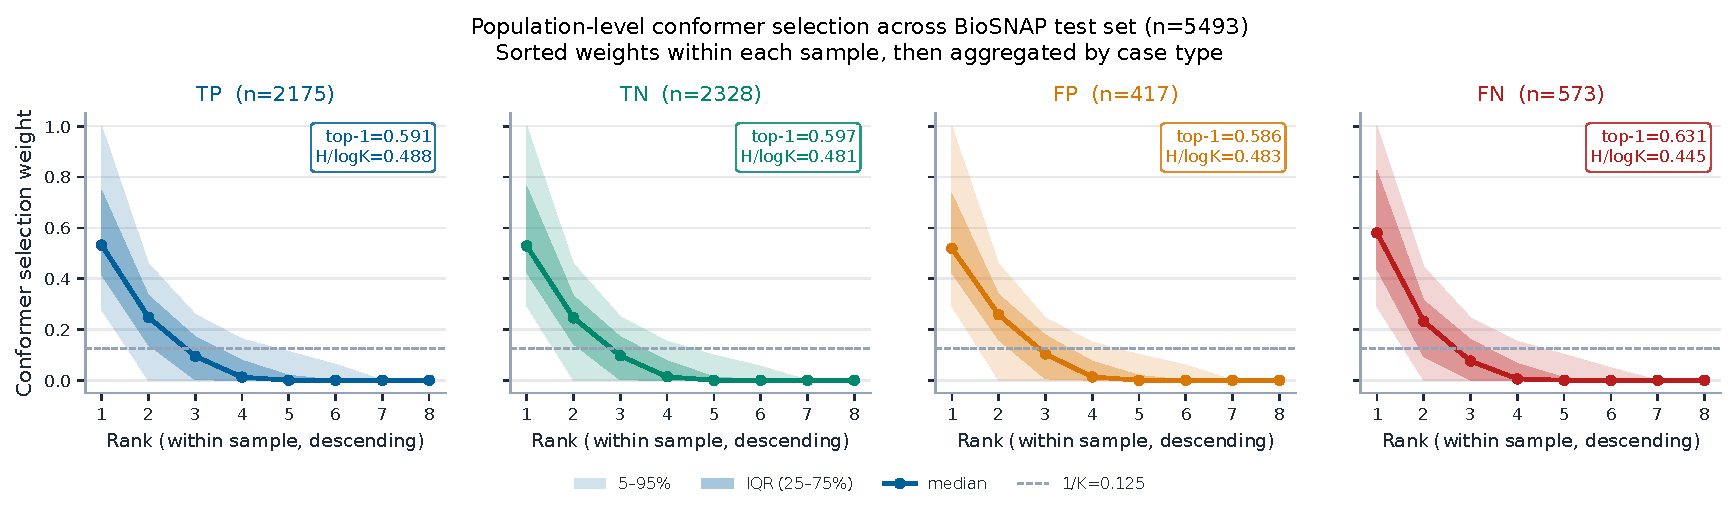
\includegraphics[width=0.98\textwidth,height=0.78\textheight,keepaspectratio]{figures/interpretability_conformer_weights.pdf}
\caption{High-resolution version of the main-text interpretability figure. For each BioSNAP test pair, the eight conformer weights are sorted within the sample and summarized by prediction group; solid curves are medians, dark bands are interquartile ranges, and light bands are the 5--95\% ranges.}
\label{fig:si_interpretability_conformer_weights}
\end{figure}
\clearpage

\FloatBarrier


\end{document}
